\documentclass{article}

\PassOptionsToPackage{numbers, compress}{natbib}

\usepackage[preprint]{neurips_2021}

\bibliographystyle{abbrvnat}

\usepackage[utf8]{inputenc}
\usepackage[T1]{fontenc}
\usepackage{hyperref}
\usepackage{url}
\usepackage{booktabs}
\usepackage{amsfonts}
\usepackage{nicefrac}
\usepackage{microtype}
\usepackage{xcolor}
\usepackage{amsmath}
\usepackage{amssymb}
\usepackage{enumitem}
\usepackage{mathrsfs}
\usepackage{graphicx}
\usepackage{scrextend}
\usepackage{hyperref}
\usepackage{tikz}
\usepackage{bm}

\title{DINO Methods for Style Transfer}

% The \author macro works with any number of authors. There are two commands
% used to separate the names and addresses of multiple authors: \And and \AND.
%
% Using \And between authors leaves it to LaTeX to determine where to break the
% lines. Using \AND forces a line break at that point. So, if LaTeX puts 3 of 4
% authors names on the first line, and the last on the second line, try using
% \AND instead of \And before the third author name.

\author{
	Sacha Goldman \\
	Department of Computer Science\\ 
	Department of Mathematics\\
	University of Toronto\\
	Toronto, ON M5S 1A1 \\
	\texttt{sacha.goldman@mail.utoronto.ca} \\
	\And
	Yuchong Zhang \\
	Department of Computer Science \\
	Department of Mathematics \\
	University of Toronto \\
	Toronto, ON, M5S 1A1 \\
	\texttt{yuchongz.zhang@mail.utoronto.ca} \\
	\And
	Shirley Wang \\
	Department of Computer Science \\
	University of Toronto \\
	Toronto, ON M5S 1A1 \\
	\texttt{shirlsyuemeng.wang@mail.utoronto.ca} \\
}

\begin{document}

\maketitle

\begin{abstract}
We apply DINO \cite{DINO}, a self-supervised learning method that captures feature representations of input images, to style transfer by extending StyTr2 \cite{ImageStyleTransformer}, a style transfer transformer that renders images with artistic style, and explore the nature and robustness of the resulting model. We explore using the vision transformers pretrained with the DINO method to encode image style, and we also explore apply the DINO training methods directly to StyTr2. We discuss the relative qualitative and quantitative performance of our new models compared to the state of the art.
\end{abstract}

\section{Introduction}
Style transfer is the problem of changing an image's artistic style while maintaining its ``content'', namely the object it depicts. Conventional models use a CNN to extract features from an image, take in another image indicating the desired artistic style, and attempt to apply that style to the features of the original input image. However, it has been shown that due to the locality resulting from shared weights, CNN based models struggle to capture the global information of input images and suffer from feature losses \cite{ImageStyleTransformer}. To resolve these issues, models that use transformers instead of CNNs for feature and style extraction have been proposed and show better results, like StyTr2 \cite{ImageStyleTransformer}. This model takes in a content image and a style image, then uses two transformer encoders to capture the content and style, then renders the content with that style using a transformer decoder. In our project, we will substitute the DINO method and models from \cite{DINO} for the encoder components and explore the effects on style transfer. The DINO method is good at extracting content even if the input images are distorted or partial, so in particular, we will implement the models and conduct experiments to explore the following questions:
\begin{enumerate}
	\item Does DINO's ability to capture an image's global property from local pieces give it more robustness as a style encoder?
	\item Are the results of this new style transfer method better than previous methods?
\end{enumerate}

\section{Related Works}

\cite{DINO} came up with a new self-supervised learning method, named DINO (for Knowledge Distillation with No Labels) that aims to create better feature representations from its inputs by adopting a teacher-student paradigm. The student gets multiple difficult views (lots of augmentation), called the local views of the image while the teacher gets an easy view (minimal augmentation), called the global view. Then the student is trained to aim for the same feature representation through cross entropy loss. Their experimental results found that the vision transformer's class token contained explicit information about the segmentation of objects in images, while also performing as very accurate classifiers. In this project, we aim to apply the better feature representation that the DINO method yields (over supervised vision transformers), to the domain of image style transfer.

Self-supervised learning is a common technique used in style transfer, due to the obvious lack of target images available for a task of this nature. It becomes necessary to find ways for the model to supervise its own outputs. Usual methods \cite{CNNStyleTransfer} involve checking the outputs of VGG for consistency in style and context. \cite{ImageStyleTransformer} proposes using vision transformers for this task, using two transformer encoders (one for content, one for style), and one transformer decoder. Transformers have been a hot rising topic in computer vision, and they claim that their method of using transformers for style transfer results in decreased content leak, as well as achieving unbiased stylization.

It is integral for there to be good feature representations of the content and style to construct a good style-transferred image. We believe that making use of pretrained DINO ViT models, as well as using the DINO method itself during training, can help achieve this.

\section{Methods}

\subsection{DINO Pretrained ViT Content Encoder}

The DINO paper provided their Vision Transformers that were trained using their proposed method. We attempted to use these models as a starting point for the content and style encoders of the model in three different ways: A) Freezing the weights for both the content and style encoders, B) Freezing only the weights for the content encoder, and C) letting both the content and style encoders train with the rest of the network.

\subsection{DINO Training the Style Encoder}

To translate the success of DINO training on classification to style transfer we modify the algorithm and architecture of StyTr2. Now instead of simple transformer for the style encoder, there is a teacher style encoder $SE_t$ and a student style encoder $SE_s$, both using the architecture from \cite{ImageStyleTransformer}. We use the extra encoder to force the student to learn distillations of the original images. Because style is a global property of an image, we applied this only to the style encoder and left the content encoder $CE$ as it was in \cite{ImageStyleTransformer}. 

To train this model, as in \cite{DINO}, from the original style image we generate two slightly modified global views of the image $(I_s)^g_1$ and $(I_s)^g_2$ as well as a collection more heavily modified local views, with the set of all views denoted $V$. The student is passed all the views whereas the teacher is only passed the global views. We then calculate 
\begin{align}
	\mathcal L_d &= \sum_{I \in \{(I_s)^g_1, (I_s)^g_2\}} \sum_{I' \in V - \{ I \}} H(SE_t(I), SE_s(I'))
\end{align} 
Where $H(a,b) = -a \log (b)$. This loss is what forces our student style encoder to learn these distilled representations. We can average $SE_s((I_s)^g_1)$ and $SE_s(I_s)^g_2$ to get the encoded style, and we can take $CE(I_c)$ to get the content. From this we can generate $I_o$, the output image, using the decoder $D$. We can also pass the encoded style to both inputs of $D$ to get $I_{ss}$ and similarly with the encoded content to get $I_{cc}$. Now we can use $\mathcal L_c$, $\mathcal L_s$, $\mathcal L_{id1}$,$\mathcal L_{id2}$ from \cite{ImageStyleTransformer}. We can then combine these into the final loss
\begin{align}
	\mathcal L &= \lambda_d \mathcal L_d + \lambda_c \mathcal L_c + \lambda_s \mathcal L_s + \lambda_{id1} \mathcal L_{id1} + \lambda_{id2} \mathcal L_{id2}
\end{align}
where the $\lambda$'s are weightings. We call this model D). We can train this using gradient based optimization, except the weights of the teacher are not updated by the gradient. The weights of the teacher are an exponential moving average of the students weights. 

We also define model E) where we modify (1) to
\begin{align}
	\mathcal L_d &= \sum_{I \in \{(I_s)^g_1, (I_s)^g_2\}} \sum_{I' \in V - \{ I \}} H(D(SE_t(I), CE(I_c)), D(SE_s(I'), CE(I_c))).
\end{align}
Hoping that calculating the loss after the decoder will weigh the most relevant differences between the student and teacher higher. Relevant meaning making a greater difference to the final issues.

\section{Experiments}

\subsection{Implementation Details}

MS-COCO [cite] is used as the content dataset and WikiArt [cite] is used as the style dataset. In the training stage,
all the images are randomly cropped into a fixed resolution of 256 x 256, while any image resolution is supported at the test time. We used the Adam optimizer [cite] and a warm-up adjustment strategy [cite] is used. Our GPU is not as big as the one used in the original paper, so while we could not train with their batch size, we modified the learning rate decay, number of iterations trained, and gradient accumulation steps to mimic the original's training process of a batch size of 8 for 160,000 iterations. Gradients are also clipped to a maximum norm of 10 to prevent exploding gradients.

\subsection{Qualitative Evaluation}

\begin{center}
\begin{figure}
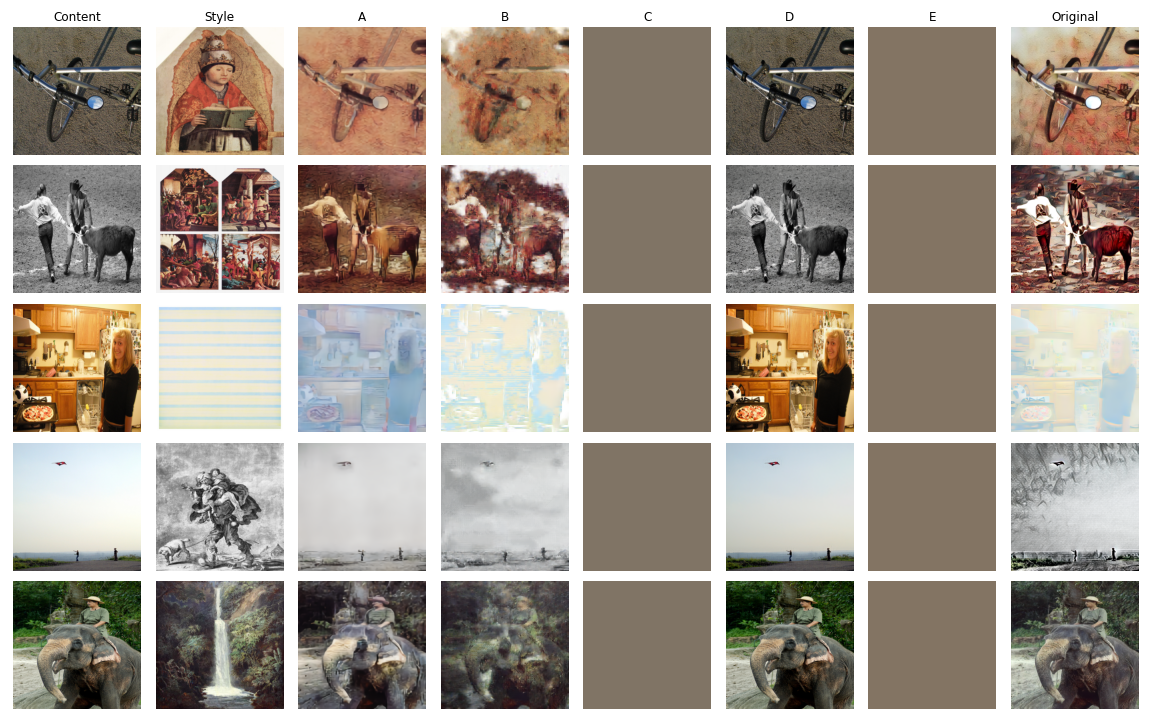
\includegraphics[width=14cm]{comparison}	
\caption{Style transfer results across different experiments.}
\label{comparison}
\end{figure}
\end{center}

In both experiments A and B, we can see that as training progresses, the model gradually learns to render the content image to the style of the style image. But in both cases, certain details of the objects depicted in the content image are lost. Experiment A seems to have less feature losses while experiment B produces style-transferred images that are closer to what the original style transferer produces (columns A, B, Original, figure \ref{comparison}). For experiment A, we can see both the content and style losses decrease over time. Meanwhile, experiment B has a decreasing style loss but its content loss first decreases and then increases before oscilating more.

Experiment C failed to learn style transfer. At the beginning of the training, it renders each content image with a color that roughly matches the style image, but over time, it started to copy the content image while completely ignoring the style image. After 300k iterations, the model abruptly started to output single-colored images regardless of what the content and style images are (column C, figure \ref{comparison}). As expected, the model's content loss decreases as it learns to copy the content images exactly and the style loss see no improvements.

During its training process, experiment D seems to be slowly learning to replicate the content image while not paying much attention to the style image. The resulting outputs started as poor-quality content images, but they slowly converged to the content images with some slight color variations (column D, figure \ref{comparison}). We see the content loss slowly decreases as training progresses while the style loss oscilates and shows no signs of improvement.

Finally, experiment E also failed. In early stages of the training, the model renders the content with many colored vertical strips and many features were lost. Eventually, the model started to output single-color images (column E, figure \ref{comparison}). We see no improvements in the style loss while the content loss abruptly drops at around 250k epochs when the model outputs became mostly single-colored images, then the content loss starts to oscillate again.

\subsection{Quantitative Evaluation}

\section{Conclusion}

\medskip

% Our current sources
\nocite{*}

\bibliography{bib}

\end{document}